\documentclass[../../submission.tex]{subfiles}
\begin{document}
\section{Result}
A primary objective of this study was to ascertain the impact of the
natural language interface on the search behavior and user satisfaction of the users in comparison to conventional search systems.
We hypothesize that users will evaluate the system employing artificial intelligence more effectively than they would a conventional system.
The reason for this is that users will have more ease of use when filtering content, as opposed to the more difficult experience they face when using a conventional system.
We also hypothesized that the utilization of filters will persist, despite the presence of natural language, which provides a predetermined framework. 
This is due to the fact that the website currently relies on filters to narrow down content.
As previously stated, an NLI has been implemented and a website for dogs has been developed to conduct a user study.


\subsection{User Satisfaction \& Behavior(RSQ1)}
As illustrated in Figure \ref{fig:result_KI}, all participants who contributed to the study 
expressed satisfaction with the outcomes generated by the AI.  A considerable 
proportion of the users, amounting to 30\%, expressed profound satisfaction with 
the outcomes, attributing this positive sentiment to the effective comprehension 
of their intentions by the artificial intelligence system.

\begin{figure}[h]
    \centering
    \begin{minipage}{0.45\textwidth}
        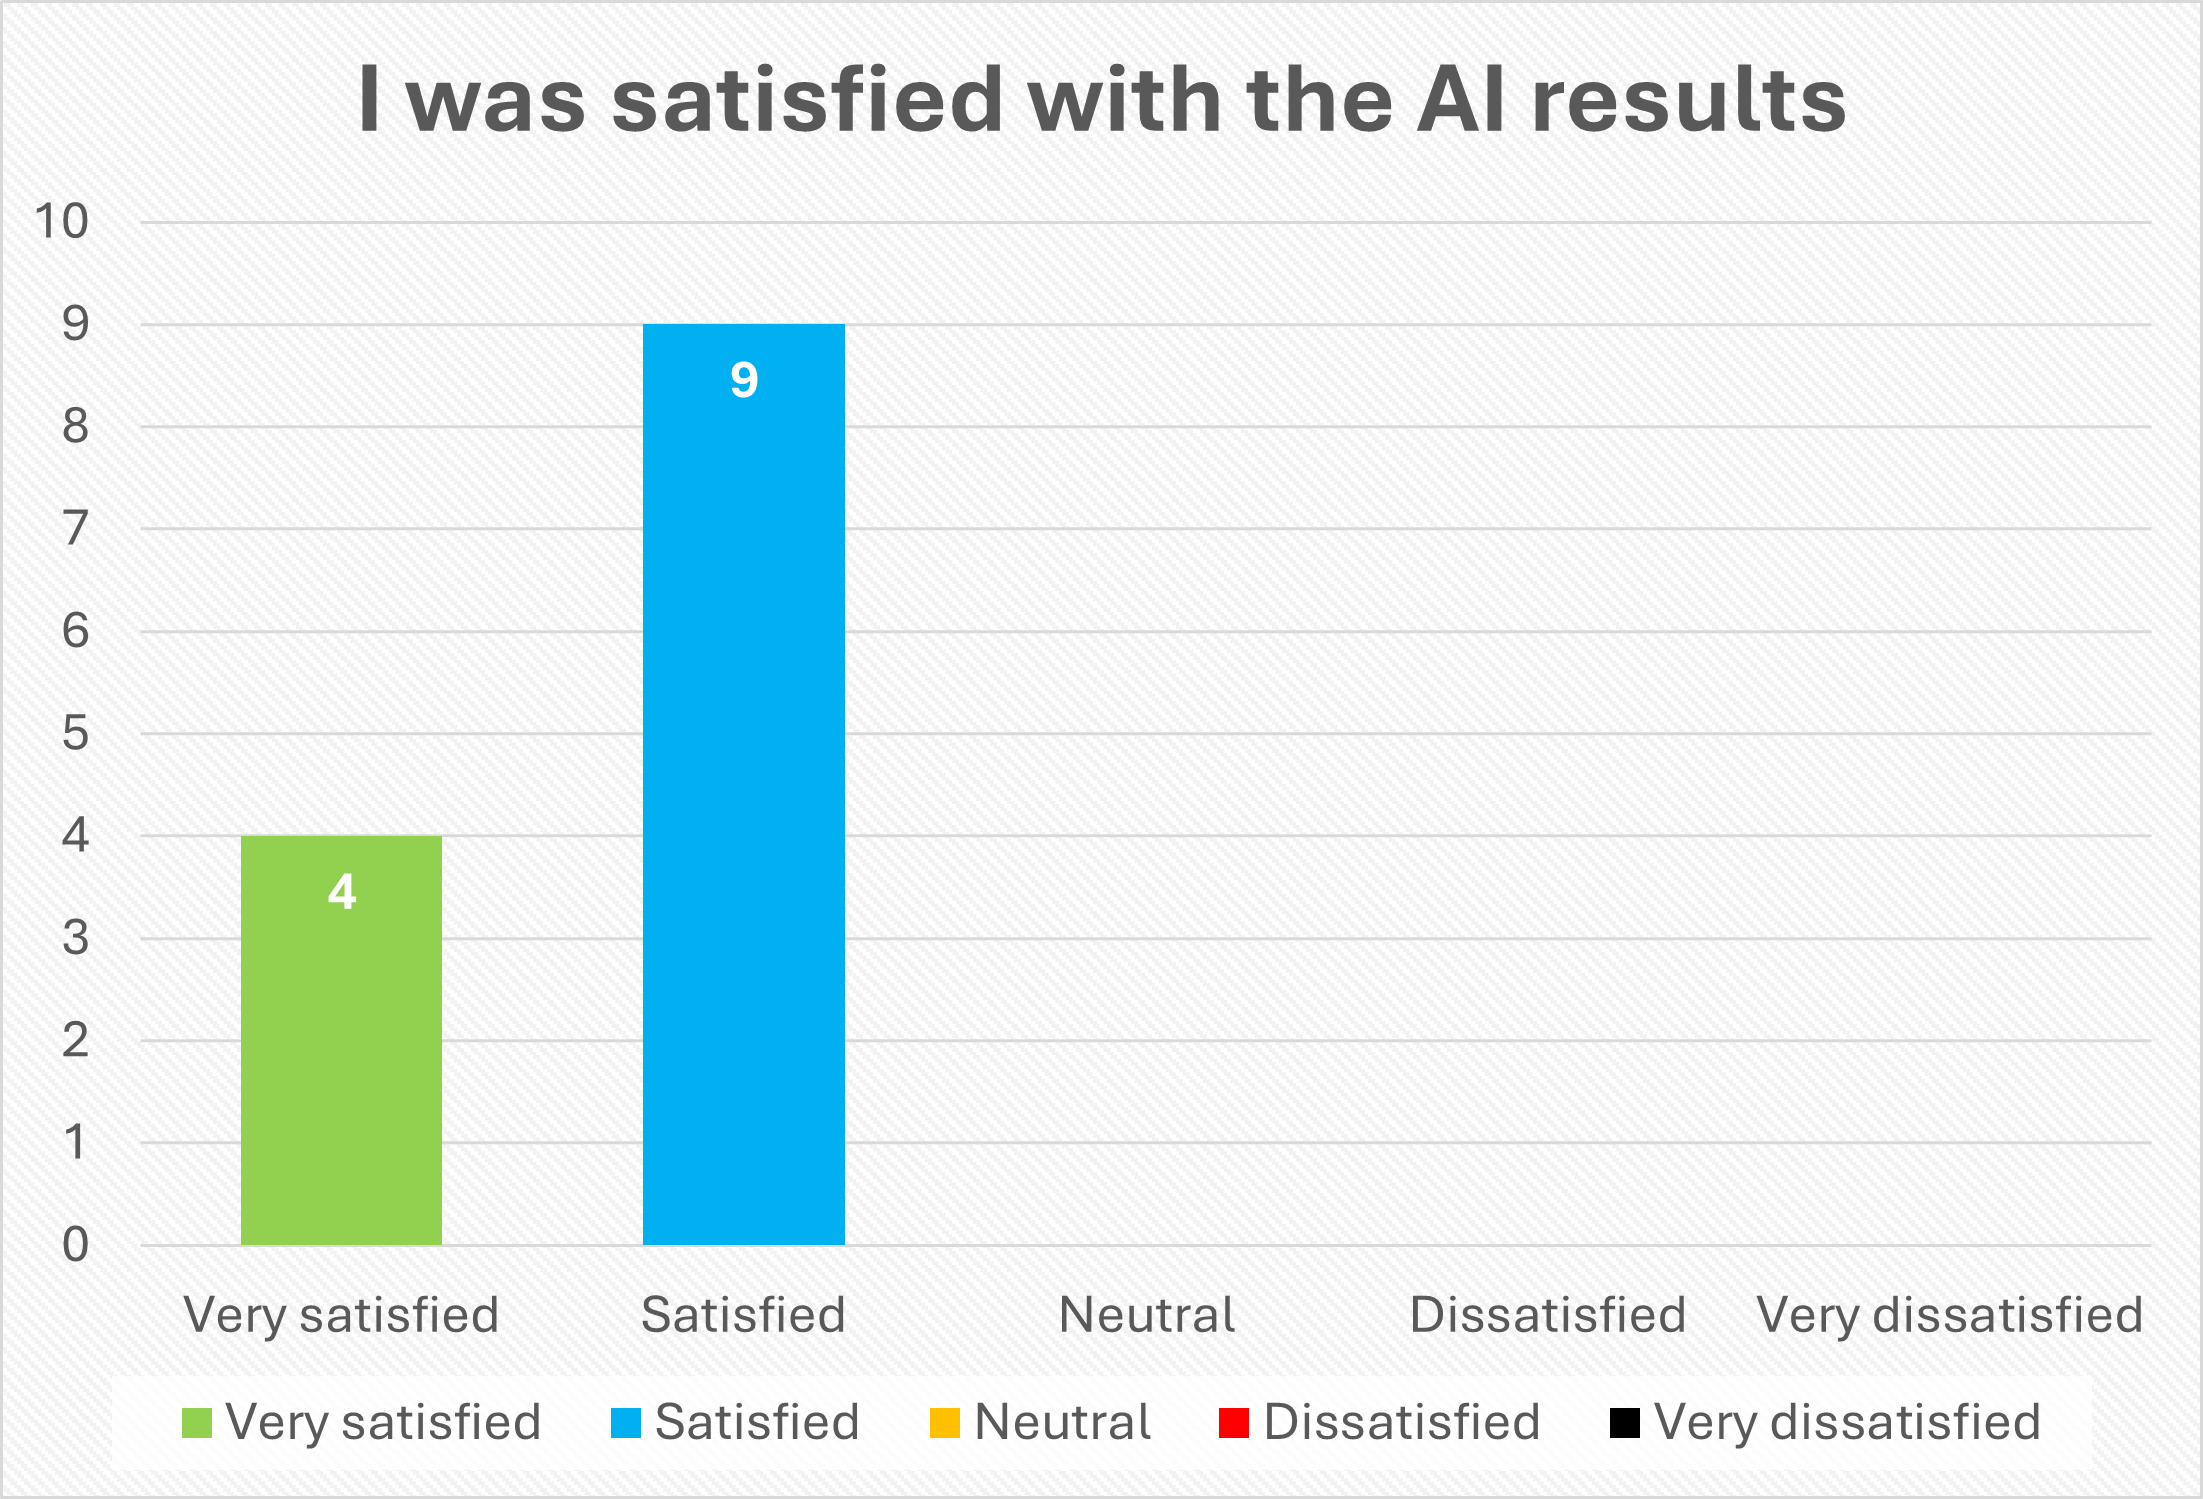
\includegraphics[width=\textwidth]{images/result_ki}
        \caption{The users' rating regarding the satisfaction of the results displayed by the AI. As can be seen in the picture, the proponents were very satisfied with the results of the AI.}
        \label{fig:result_KI}
    \end{minipage}
    \hfill
    \begin{minipage}{0.45\textwidth}
        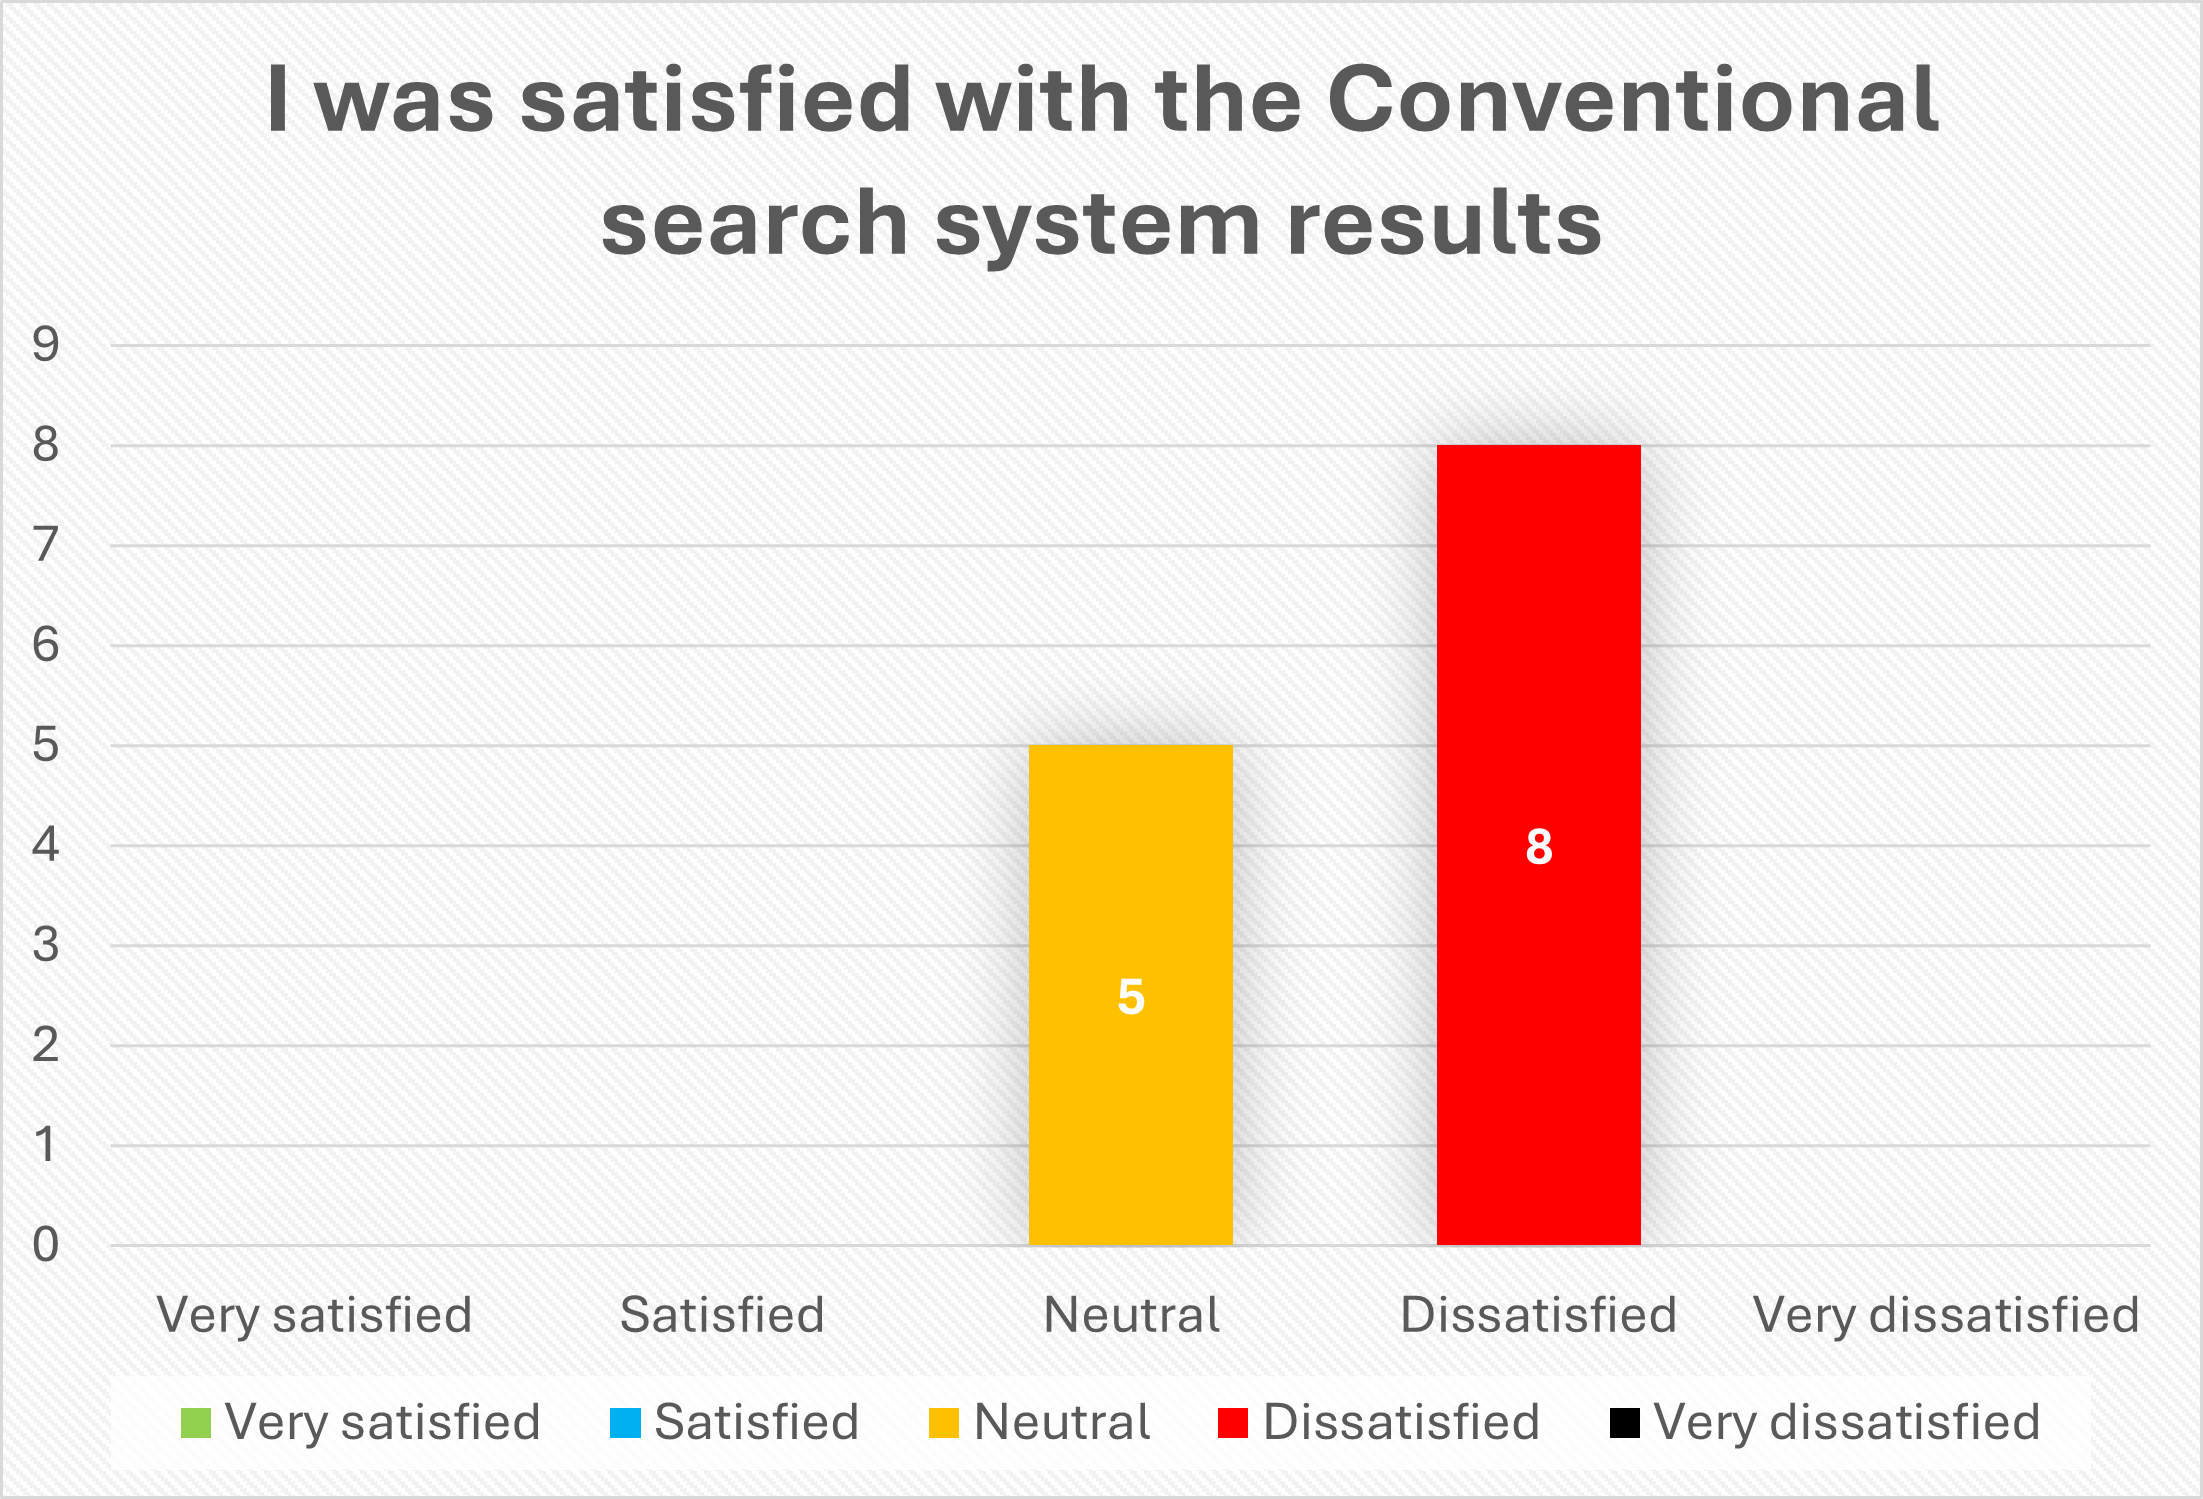
\includegraphics[width=\textwidth]{images/result_konv}
        \caption{The evaluation of the users regarding the satisfaction with the result displayed by the conventional system. The picture shows that they were not satisfied with the results displayed by the conventional system.}
        \Description{}
        \label{fig:result_Konv}
    \end{minipage}
\end{figure}

A further aspect that was found to be well-received by the users was the ability of the KI to automatically 
manage tip errors and synonyms. As illustrated in Figure 10, the search for a Dachshund 
is demonstrated. However, a synonym is employed in place of the Dachshund. In this 
particular instance, the search is for a Wiener Dog. As the image illustrates, the AI 
interprets the synonym correctly. This demonstrates a capability that is absent in the 
conventional system. 

\begin{figure}[h]
    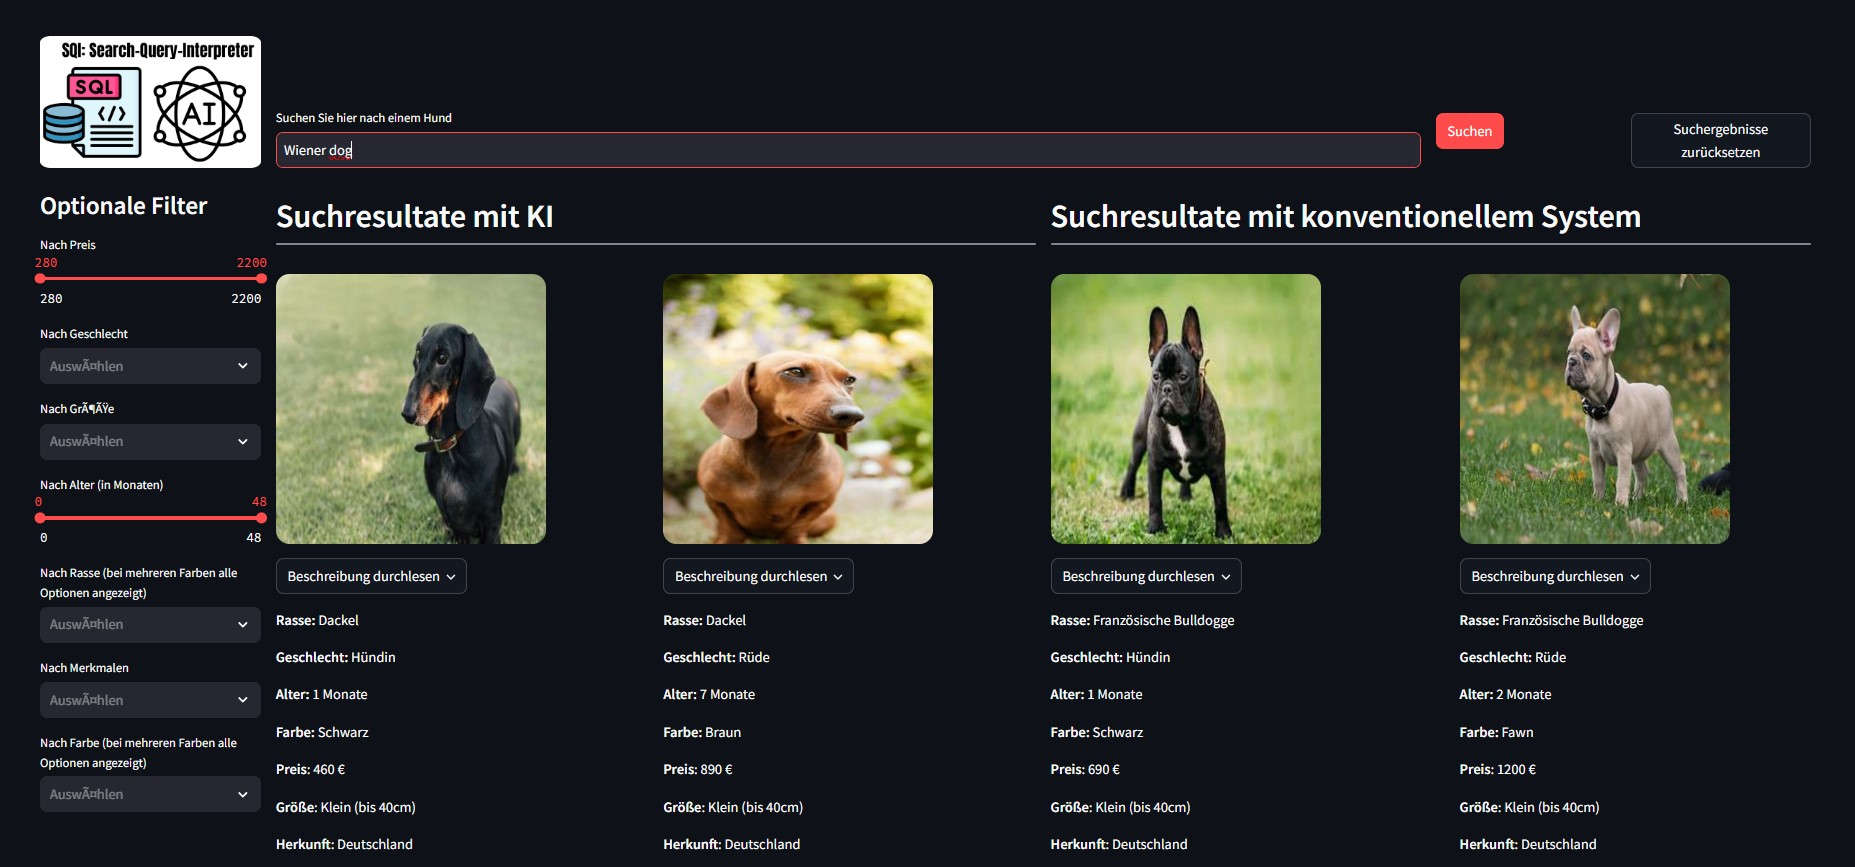
\includegraphics[width=\textwidth]{images/wiener_dog}
    \caption{Here the search is for a dachshund, but instead of entering dachshund, a synonym is used to show that the AI can also interpret it}
    \Description{}
    \label{fig:wiener_dog}
 \end{figure}



A review of the satisfaction levels observed in conventional systems clearly 
indicates a preference for AI, as demonstrated in Figure \ref{fig:result_Konv}. However, it should 
be noted that the study revealed a notable observation: the presence of a decline 
in the utilization of filters by users, coinciding with the enhanced comprehension 
of user intentions by the AI system. This phenomenon led to the suboptimal performance
 of the conventional system in comparison to the AI-based alternative. 
 Therefore, it is important to consider the potential for a filter bias, 
 which could explain the users' discontent with the results.
 It is possible that the results would have been more favorable had the experiment 
 been conducted differently.


 It was not anticipated that the users would adapt to the new 
 system so rapidly, leading to a decrease in the usage of filters.
 Had the expectation been present, the implementation of a filter counter would 
 have been a possibility, with the objective of determining the actual utilization of the filters.
 A more thorough examination would have been beneficial in order to ascertain the extent of the alterations in search behavior.

 \subsection{Importance of Filters}
A further aspect that emerged from our user study is the significant relevance 
attributed to the filters, despite the participants' awareness that artificial 
intelligence could potentially substitute for their functionality.

 \begin{figure}[h]
    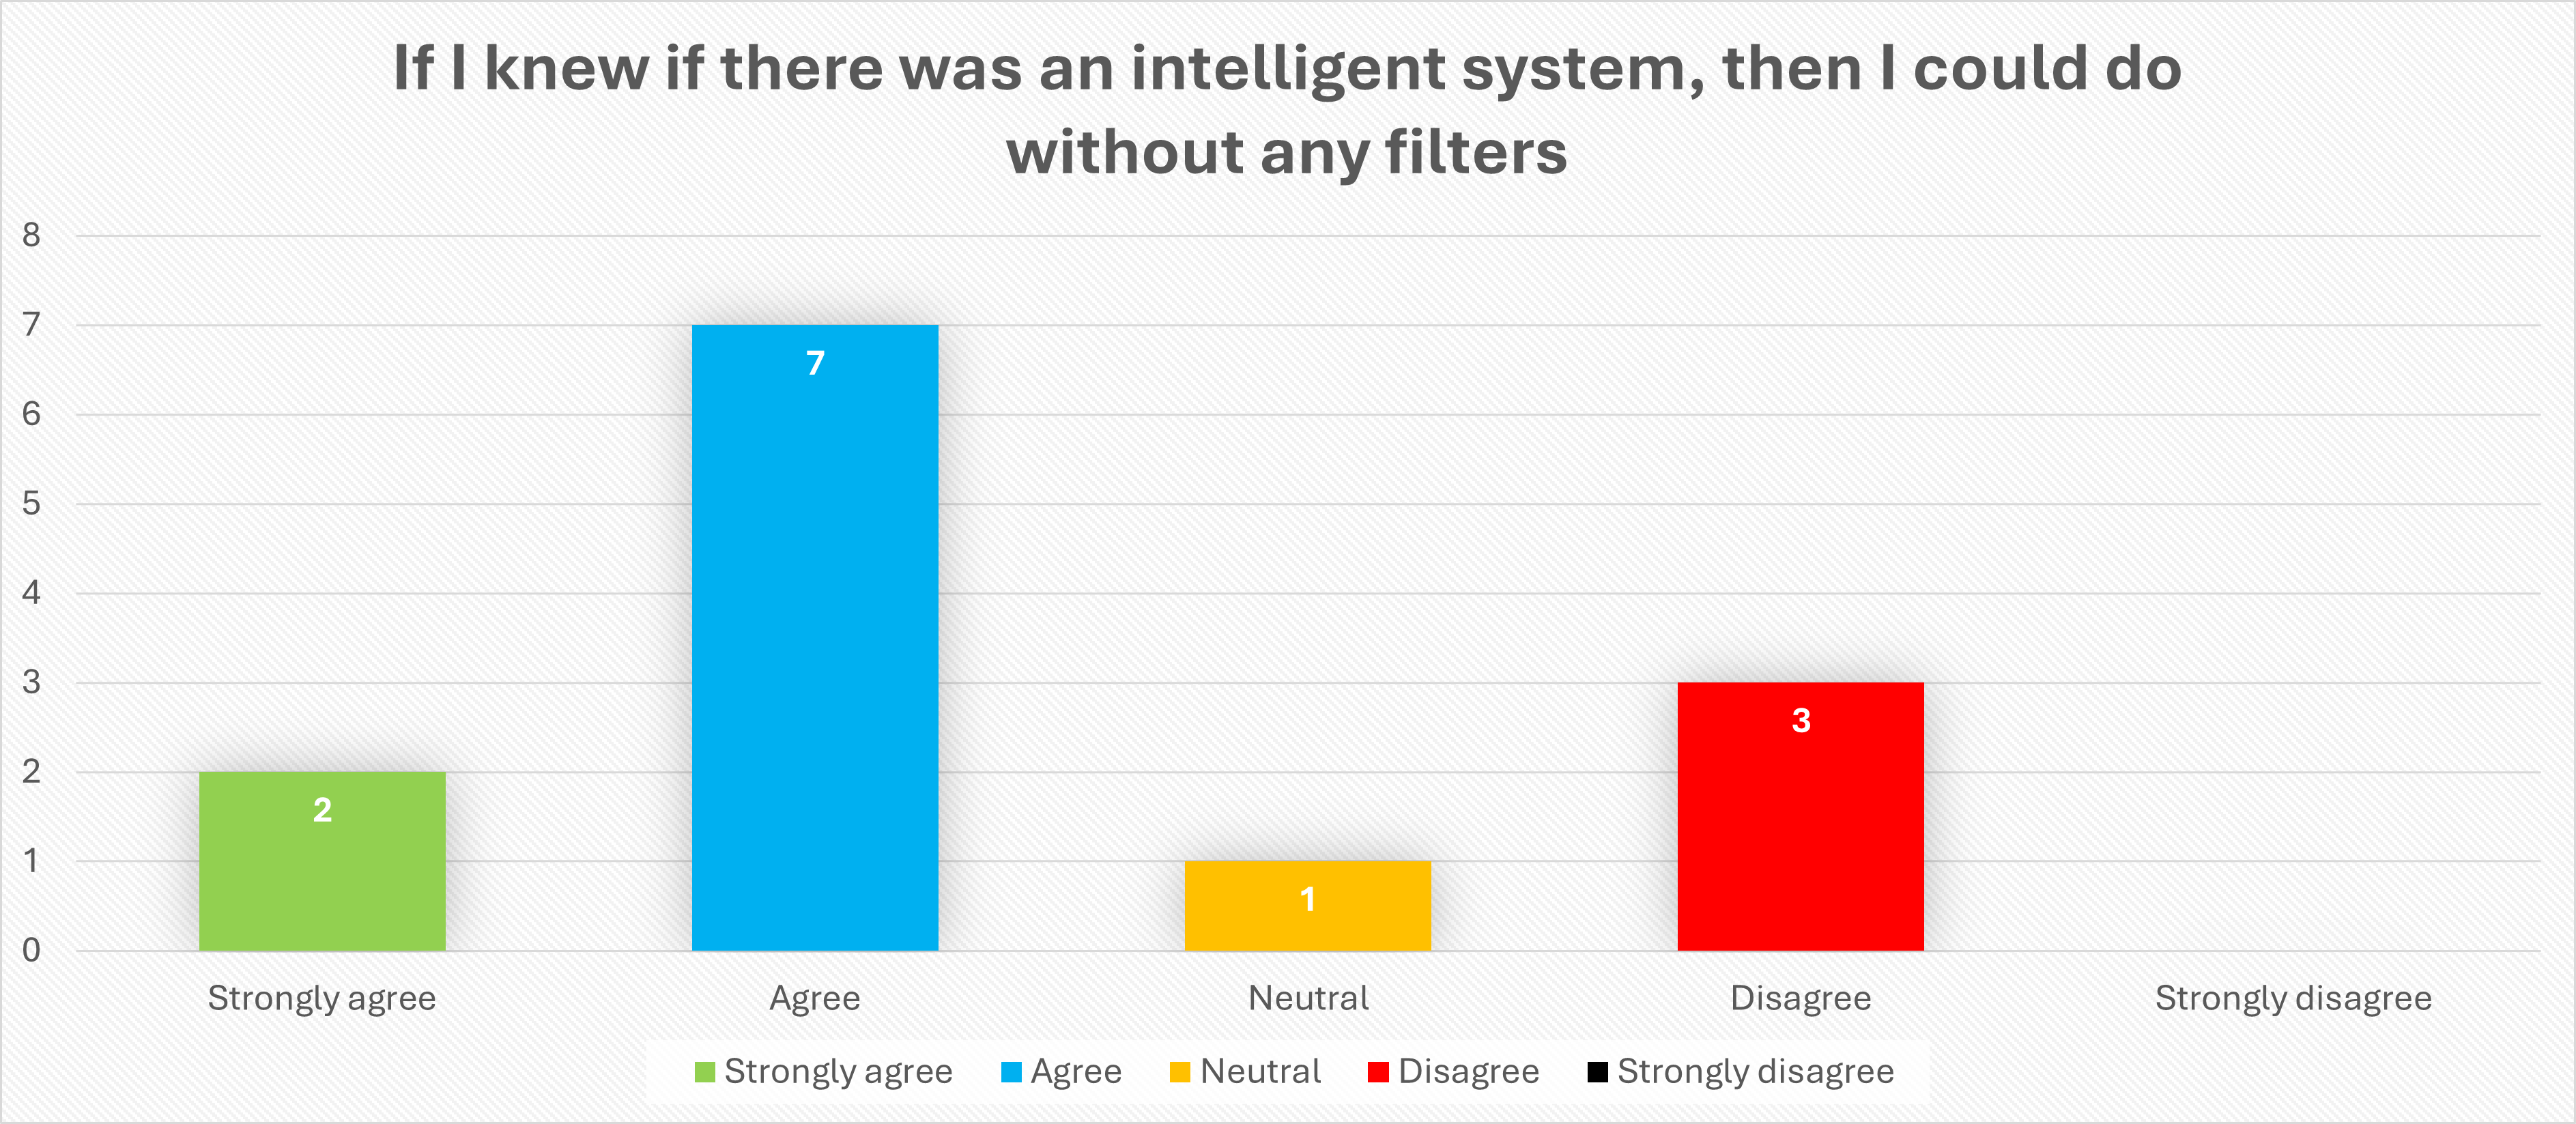
\includegraphics[width=\textwidth]{images/without_filter}
    \caption{After the users have used the system, they should state whether they would manage without the filter}
    \Description{}
    \label{fig:without_filter}
 \end{figure}

 As illustrated in Figure \ref{fig:without_filter} , there is considerable variation in opinion among 
 the users. Approximately 70\% of users affirm that, should such a system be 
 in place, the absence of filters would be acceptable to them. Nonetheless, 
 approximately 20\% of respondents indicated a preference for maintaining web 
 filters, even in the context of a system that incorporates these filters. 
 The underlying reason for this phenomenon is that users prefer to utilize visual 
 filters, such as sorting or price filters, rather than using it through tipping. 
 The proponents indicated that the process of establishing the price filter is 
 straightforward. They noted that this is due to the ability to swiftly determine 
 the range of products in question, as opposed to the more cumbersome method of 
 manual calculation. Five of the propants who expressed agreement also indicated 
 a desire for additional practical filters, like the previously mentioned filters, 
 such as price and sorting. This additional desire for filters is the reason why 
 they did not strongly agree. Therefore, even if a system with AI is used, it is 
 important to maintain filters.


 \subsection{Good ways to fix query (RSQ3)}
 A significant challenge arises from the lack of transparency in artificial intelligence systems, 
 particularly regarding the underlying processes and algorithms that generate results. 
 The optimization of SQL queries can be achieved through various methods. 
 One such approach entails enhancing the initial query. However, this approach may present a challenge, as it requires that the user comprehend the erroneous interpretation of the query. 
 To optimize the request, it is first necessary to develop a more profound comprehension of the underlying system. 
 In this regard, the method for enhancing the user experience proposed in \cite{popescuEtalTowardsTheoryOfNaturalLanguage} may be applicable. 
 This method enables the user to select from among various options.  


 Nevertheless, in order to consider the user preferences, a survey was conducted among the participants to ascertain how they would prefer to be assisted in the event that their preliminary search request did not align with their actual needs.
 The proponents advanced a number of intriguing concepts. For instance, the potential exists for the artificial intelligence to adjust the filters 
 based on the user's search history. As illustrated in Figure \ref{fig:filter}, the potential appearance of the phenomenon is 
 demonstrated. In this instance, the filter is dynamically adjusted. Therefore, the user is able to ascertain 
 which filters the KI utilizes and, consequently, identify the potential origin of an error. Therefore, the user 
 has the option of either utilizing the filter to resolve the issue or adjusting the initial search query.
 
 \begin{figure}[h]
     \centering
     \begin{minipage}{0.35\textwidth}
         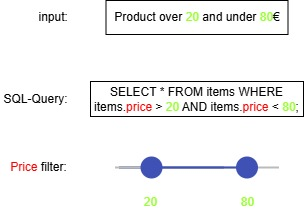
\includegraphics[width=\textwidth]{images/filter}
         \caption{Here the user can see how the filter is adapted to the user's input. The user can see here exactly what the AI is doing wrong.}
         \Description{}
         \label{fig:filter}
     \end{minipage}
     \hfill
     \begin{minipage}{0.55\textwidth}
         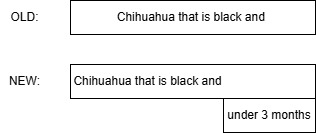
\includegraphics[width=\textwidth]{images/vorschlag}
         \caption{Here the user is informed by the AI if the features are not combinable. Instead, the AI suggests other features that can be combined.}
         \Description{}
         \label{fig:suggestions}
     \end{minipage}
 \end{figure}
 A further potential avenue for enhancing the efficacy of the user's 
 outcomes is the implementation of an artificial intelligence system that can 
 evaluate the combinability of diverse features during the user's input phase. 
 In such a case, it is essential that the user be alerted to this possibility. 
 As demonstrated in Figure \ref{fig:suggestions}, the initial state is displayed, denoting the current 
 state of affairs.The subsequent version has been enhanced to alert the user to the 
 absence of products for a given combination of features. In this instance, the 
 "under 2 months" feature is distinctly emphasized, as it does not result in any products. 
 Therefore, the user has the capacity to modify the preliminary search query and discern the 
 elements that are not compatible. The integration of this concept with the search function 
 can result in the automatic generation of suggestions for relevant features. This concept is 
 further illustrated in Figure \ref{fig:suggestions}.
 
 A further point to be considered is the potential for the AI to present analogous 
 products in the event that the search yields minimal results. A relevant example  
 would be a search for dogs that are of medium size. In the event that the available 
 results are limited, the artificial intelligence could be programmed to display dogs of 
 smaller stature.
 


\end{document}